% -----------------------------------------------------------------------------
% Metodologia
% -----------------------------------------------------------------------------

\chapter{Metodologia}
\label{chap:metodologia}
Com o objetivo de criar aplicações que simulem cada uma das camadas do modelo TCP/IP, foram escolhidos cinco protocolos para serem implementados. Da camada de aplicação o protocolo HTTP, utilizado para comunicação de um sistema final e um servidor Web, permitindo assim navegação pela Internet, será implementado. Da camada seguinte, a de Transporte, devido a sua importância, os dois principais protocolos serão implementados, o protocolo de transporte confiável, TCP, e o não confiável, UDP.
 
Os seguimentos recebidos da camada de transporte deverão ser tratados na camada de internet pelo protocolo IP fazendo uso do roteamento o qual, por sua vez, deverá entregar o pacote resultante para camada de Enlace. Esta terá o protocolo Ethernet simulado, complementado do protocolo ARP para tradução do endereço IP para MAC, possibilitando assim o envio do quadro para o host destino.

A Figura \ref{fig:objetivo} mostra a formulação implementada neste trabalho, representando o funcionamento da pilha de protocolos quando uma aplicação cliente, no caso o browser, faz uma requisição HTTP ao servidor. A arquitetura cliente/servidor foi utilizada para promover a interação entre as camadas, assim elas conversam entre si através de sockets, onde as portas são representadas pelo caminho aberto em cada camada e as mensagens são representadas pelas setas: vermelha ilustrando a mensagem de requisição, e azul a reposta mandada pelo servidor.


\begin{figure}[H]
	\centering
    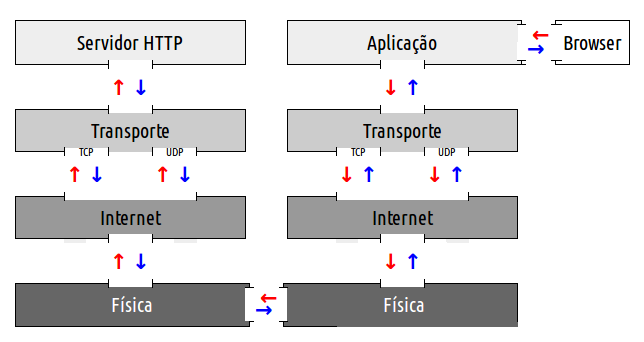
\includegraphics[width=0.80\textwidth]{04-figuras/Esquema.png}
    \caption{Esquema da arquitetura desenvolvida}
    \label{fig:objetivo}
\end{figure}

Cada camada foi implementada de forma independente, e a cada etapa os dados referentes à PDU são exibidos para, assim, manter a transparência objetivada para a utilização deste sistema como ferramente de ensino. Estes dados são estruturados de acordo com os respectivos padrões definidos pela RFC.

Objetivando a melhor forma de implementação, considerando a simplicidade e bibliotecas disponíveis para acesso baixo n\'ivel \'a rede, a linguagem escolhida foi o Python, vers\~ao 2.7. O planejamento teve como objetivo permitir a interaç\~ao entre camadas e testes a cada etapa do desenvolvimento. Desta forma o primeiro m\'odulo desenvolvido foi referente a camada F\'isica para garantir a transmiss\~ao de mensagens entre hosts. Utilizando este m\'odulo como base foram desenvolvidos, na seguinte ordem, os m\'odulos simuladores referentes \'a camada de Aplicaç\~ao, Transporte e Internet.
